\chapter{Supercargas, cierre y superspacio}

\lectureoverview{La supersimetría es difícil, no porque sus reglas sean numerosas, sino porque estas reúnen ideas que la física ordinaria mantiene separadas. Empezamos con variables de Grassmann, cuyos elementos impares anticonmutan y cuyas funciones se truncan tras un número finito de términos. El álgebra de sus derivadas proporciona entonces el modelo para los generadores de simetría impares. Un oscilador bosónico y uno fermiónico dan lugar a las supercargas más sencillas: su anticonmutador es el hamiltoniano, de modo que el intercambio de bosones y fermiones es inseparable de las traslaciones temporales. La misma álgebra puede representarse geométricamente mediante traslaciones en direcciones de Grassmann de un espacio-tiempo ampliado llamado superspacio.}

\section{Por qué hay que retroceder antes de avanzar}

La supersimetría es una de las construcciones más abstractas de la física. Se parece a las rotaciones y las traslaciones porque es una simetría, pero no cabe en el espacio-tiempo ordinario sin ampliar lo que entendemos por coordenada. Sus parámetros naturales son cantidades de Grassmann: objetos que pueden sumarse y multiplicarse, pero que anticonmutan en vez de conmutar.

Por eso no sería útil abordar directamente el álgebra final. Primero haremos manejable la aritmética impar; después recordaremos cómo se organizan las simetrías continuas ordinarias, y solo entonces combinaremos ambas ideas. El recorrido es más largo, pero cada paso prepara el siguiente.

\section{El álgebra de Grassmann en la práctica}

\subsection{Elementos impares y pares}

Sean \(\epsilon_i\) generadores independientes de Grassmann. Cumplen
\begin{equation}
\epsilon_i\epsilon_j=-\epsilon_j\epsilon_i,
\qquad
\{\epsilon_i,\epsilon_j\}=0.
\end{equation}
Al tomar \(i=j\) se obtiene
\begin{equation}
2\epsilon_i^2=0,
\qquad
\epsilon_i^2=0,
\end{equation}
sobre los números reales o complejos. El generador no es cero; solo su cuadrado es cero.

Cada elemento homogéneo tiene una paridad. Un producto que contiene un número impar de generadores de Grassmann es impar, mientras que uno que contiene un número par es par:
\begin{align}
\text{odd}\times\text{odd}&=\text{even},\\
\text{odd}\times\text{even}&=\text{odd},\\
\text{even}\times\text{even}&=\text{even}.
\end{align}
Los elementos pares conmutan con los elementos homogéneos. Dos elementos impares anticonmutan. Así,
\begin{equation}
n\epsilon_i=\epsilon_i n,
\qquad
\epsilon_i\epsilon_j=-\epsilon_j\epsilon_i,
\end{equation}
cuando \(n\) es par.

Un elemento par no tiene por qué ser un número real o complejo ordinario. Por ejemplo, el producto
\(\epsilon_1\epsilon_2\) es par y nilpotente. Los números ordinarios forman la parte escalar del álgebra, mientras que los productos pares aportan otros elementos conmutativos.

\begin{classroomqa}
\audiencequestion{¿Hay alguna diferencia entre el álgebra de Grassmann y los números de Grassmann, o son lo mismo? \lecturetimestamp{00:06:45}}
\lecturerresponse{Los elementos son los números de Grassmann; el álgebra es el conjunto de esos elementos junto con sus reglas de suma y multiplicación. Por tanto, puede hablarse informalmente del mismo objeto, pero es útil distinguir entre las entidades con las que se opera y las reglas que rigen esas operaciones.}
\end{classroomqa}

\subsection{Las funciones se truncan}

Una función de una variable de Grassmann solo puede contener dos potencias:
\begin{equation}
f(\epsilon)=a+b\epsilon.
\end{equation}
No hay término \(\epsilon^2\). Con dos generadores independientes,
\begin{equation}
f(\epsilon_1,\epsilon_2)
=a+b_1\epsilon_1+b_2\epsilon_2+c\epsilon_1\epsilon_2.
\end{equation}
el desarrollo termina cuando aparecen ambos generadores. Para \(n\) generadores independientes, los monomios ordenados forman una base de dimensión \(2^n\):
\begin{equation}
1,\quad
\epsilon_i,\quad
\epsilon_i\epsilon_j,\quad
\ldots,\quad
\epsilon_1\epsilon_2\cdots\epsilon_n.
\end{equation}
\editorialnote{El resultado finito en dimensión \(2^n\) es el patrón general que subyace a los ejemplos con uno y dos generadores. También puede definirse un álgebra de Grassmann infinita, pero todos los polinomios que usamos aquí contienen solo un número finito de generadores.}

Al combinar dos generadores reales en un par complejo \(\theta,\bar\theta\), una función general puede escribirse, con un orden elegido, como
\begin{equation}
f(\theta,\bar\theta)
=a+\bar b\,\theta+\bar\theta\,b+c\,\bar\theta\theta.
\end{equation}
La barra indica la notación de par complejo que usamos aquí. Invertir el orden final cambia el signo:
\begin{equation}
\bar\theta\theta=-\theta\bar\theta.
\end{equation}

Suele ser conveniente asignar una paridad definida a toda la función. Si \(f\) es par, entonces \(a\) y \(c\) son pares, mientras que \(b\) y \(\bar b\) son impares. Si \(f\) es impar, esas asignaciones se invierten. Los coeficientes pueden pertenecer a un álgebra de Grassmann más amplia, siempre que no dependan de las variables particulares respecto de las cuales desarrollamos la función.

\begin{classroomqa}
\audiencequestion{¿Se puede introducir una variable de Grassmann en funciones trigonométricas u otras funciones analíticas? \lecturetimestamp{00:11:06}}
\lecturerresponse{Sí, pero la serie de potencias se trunca enseguida. Para un generador impar,
\[
\sin\epsilon=\epsilon,\qquad
\cos\epsilon=1,\qquad
e^\epsilon=1+\epsilon.
\]
Se conservan los nombres habituales, pero hay tan pocas potencias que las funciones no pueden adquirir la complejidad analítica acostumbrada.}
\end{classroomqa}

\section{Derivar es llevar la cuenta de los signos}

Usaremos una derivada izquierda de Grassmann. Sus reglas locales definitorias son
\begin{equation}
\partial_\theta a=0,
\qquad
\partial_\theta(\theta B)=B,
\end{equation}
cuando \(a\) y \(B\) no dependen de \(\theta\). Antes de derivar, llevamos el \(\theta\) pertinente a la izquierda. Cada vez que pasa junto a otro factor impar, cambia el signo.

Por ejemplo, si \(b\) es impar,
\begin{equation}
b\theta=-\theta b,
\qquad
\partial_\theta(b\theta)=-b.
\end{equation}
No hay nada misterioso en la derivada. El signo menos apareció antes de derivar, al reordenar los factores impares.

\subsection{El cálculo con dos variables}

Volvamos a
\begin{equation}
f(\theta,\bar\theta)
=a+\bar b\,\theta+\bar\theta\,b+c\,\bar\theta\theta.
\end{equation}
Supongamos primero que \(f\) es par. Entonces \(\bar b\) es impar y \(c\) es par. Al reordenar los términos que contienen \(\theta\),
\begin{align}
\bar b\,\theta&=-\theta\bar b,\\
c\,\bar\theta\theta&=-\theta c\,\bar\theta.
\end{align}
Por tanto,
\begin{equation}
\partial_\theta f=-\bar b-c\bar\theta.
\end{equation}

Si \(f\) es impar, entonces \(\bar b\) es par y \(c\) es impar. El primer término no pasa junto a ningún coeficiente impar, mientras que en el último \(\theta\) pasa junto a dos factores impares, \(c\) y \(\bar\theta\). Los dos signos se cancelan:
\begin{equation}
\partial_\theta f=\bar b+c\bar\theta.
\end{equation}

\begin{classroomqa}
\audiencequestion{¿Por qué llevan signo menos los dos términos que sobreviven en el ejemplo par? \lecturetimestamp{00:16:49}}
\lecturerresponse{El primer signo aparece al pasar \(\theta\) junto al coeficiente impar \(\bar b\). En el último término, \(c\) es par, pero \(\theta\) tiene que pasar junto a la variable impar \(\bar\theta\). En cada reordenamiento se pasa junto a un factor impar, por lo que aparece un signo menos.}
\end{classroomqa}

La respuesta depende de la convención de orden, pero las matemáticas no. Si hubiéramos empezado con \(c\theta\bar\theta\) en vez de \(c\bar\theta\theta\), el coeficiente mostrado diferiría en un signo y la fórmula de la derivada cambiaría en consecuencia.

\begin{classroomqa}
\audiencequestion{¿Podría haberse escrito el último término con \(\theta\) y \(\bar\theta\) en orden inverso? ¿Tiene el signo resultante un significado más profundo? \lecturetimestamp{00:18:50}}
\lecturerresponse{Puede escribirse en cualquiera de los dos órdenes, pero intercambiar las dos variables impares cambia el signo. Ese signo puede incorporarse al coeficiente \(c\). En esta etapa, el efecto consiste en llevar la cuenta: el orden importa, la paridad no cambia y un cambio de signo nunca convierte un objeto impar en uno par. La importancia física aparece cuando esa misma contabilidad impone la estadística fermiónica y la supersimetría.}
\end{classroomqa}

\begin{classroomqa}
\audiencequestion{¿Los coeficientes \(a,b,c\) se toman simplemente del cuerpo de los números complejos? \lecturetimestamp{00:20:47}}
\lecturerresponse{Pueden ser números complejos ordinarios cuando su paridad debe ser par, pero también pueden contener generadores distintos de \(\theta,\bar\theta\). El álgebra de interés suele incluir todos los escalares complejos junto con un conjunto elegido de generadores impares y sus productos.}
\end{classroomqa}

\begin{classroomqa}
\audiencequestion{Las derivadas de las funciones pares e impares parecen opuestas. ¿Es una simetría general? \lecturetimestamp{00:22:31}}
\lecturerresponse{No por sí sola. Los signos se deducen mecánicamente de la paridad de cada coeficiente y del número de factores impares que se atraviesan. A veces dos resultados son opuestos por casualidad, pero la regla fiable es más sencilla: cada intercambio de dos objetos impares aporta un signo menos.}
\end{classroomqa}

\subsection{La coordenada y la derivada como operadores}

Hay una analogía ordinaria instructiva. Consideremos la multiplicación por \(x\) y la derivación respecto de \(x\), actuando sobre una función arbitraria \(g(x)\). Entonces
\begin{align}
\partial_x\!\left(xg\right)&=g+xg',\\
x\partial_xg&=xg',
\end{align}
por lo que
\begin{equation}
[\partial_x,x]g=g.
\end{equation}
Como esto se cumple para toda \(g\),
\begin{equation}
[\partial_x,x]=1.
\end{equation}
Con \(p=-i\partial_x\), esta es el álgebra familiar de posición y momento, en unidades donde \(\hbar=1\).

La analogía de Grassmann usa un anticonmutador. Tomemos
\begin{equation}
f(\theta)=a+\theta b,
\end{equation}
con \(a\) par y \(b\) impar, de modo que \(f\) es par. Primero,
\begin{equation}
\theta\partial_\theta f=\theta b.
\end{equation}
En el orden inverso,
\begin{align}
\partial_\theta(\theta f)
&=\partial_\theta(\theta a+\theta^2b)\\
&=a.
\end{align}
Al sumar ambos órdenes se obtiene la función original:
\begin{equation}
\left(\partial_\theta\theta+\theta\partial_\theta\right)f
=a+\theta b=f.
\end{equation}
Por tanto,
\begin{equation}
\boxed{\{\partial_\theta,\theta\}=1.}
\end{equation}
La derivada \(\partial_\theta\) también es impar. Por eso su relación canónica con la coordenada impar es un anticonmutador.

\begin{classroomqa}
\audiencequestion{¿Se puede usar una función que contenga partes pares e impares, en lugar de asignarle una paridad definida? \lecturetimestamp{00:31:05}}
\lecturerresponse{Se pueden formar elementos no homogéneos de ese tipo, pero normalmente los cálculos se organizan en objetos homogéneos pares e impares. Una paridad definida permite determinar sin ambigüedad cada signo en un producto graduado; un objeto mixto se trata separándolo en sus partes par e impar.}
\end{classroomqa}

\begin{classroomqa}
\audiencequestion{¿Se suponía que la función de prueba \(g(x)\) era impar en el cálculo del conmutador ordinario? \lecturetimestamp{00:31:45}}
\lecturerresponse{No. Era una función ordinaria de una coordenada ordinaria conmutativa. Se introdujo únicamente para mostrar cómo se demuestra la identidad de operadores \([\partial_x,x]=1\) antes de repetir el argumento con el par de Grassmann \(\partial_\theta,\theta\).}
\end{classroomqa}

\begin{classroomqa}
\audiencequestion{¿Hay un límite para el número de generadores de Grassmann independientes? \lecturetimestamp{00:32:16}}
\lecturerresponse{No hay límite algebraico. Para \(n\) generadores, la base tiene \(2^n\) monomios, por lo que la contabilidad crece rápidamente, pero la construcción funciona para cualquier \(n\) finito.}
\end{classroomqa}

\subsection{Integración}

La integral sobre una variable de Grassmann queda definida por
\begin{equation}
\int d\theta\,1=0,
\qquad
\int d\theta\,\theta=1.
\end{equation}
En consecuencia, para \(f(\theta)=a+\theta b\),
\begin{equation}
\int d\theta\,f(\theta)=b=\partial_\theta f(\theta).
\end{equation}
Así, la integración y la derivación extraen la misma componente. Esta es la integral de Berezin. Su normalización es la única elección sencilla compatible con la invariancia ante traslaciones y con la integración por partes de Grassmann. \editorialnote{Las reglas para las componentes precisan la afirmación de la clase de que la integración y la derivación de Grassmann son la misma operación.}

\section{La simetría ordinaria como referencia}

Consideremos un grupo unitario continuo con generadores hermíticos \(G_i\). Cerca de la identidad,
\begin{equation}
U(\alpha)=\mathbf 1+i\alpha^iG_i+O(\alpha^2),
\end{equation}
donde los \(\alpha^i\) son parámetros conmutativos ordinarios. La ley de multiplicación infinitesimal queda codificada por el álgebra de Lie
\begin{equation}
[G_i,G_j]=i f_{ij}{}^{k}G_k.
\end{equation}
Las constantes \(f_{ij}{}^k\) son las constantes de estructura. El cierre significa que el conmutador de dos generadores cualesquiera es una combinación lineal de generadores que ya pertenecen al álgebra.

Para las rotaciones,
\begin{equation}
[L_i,L_j]=i\varepsilon_{ijk}L_k.
\end{equation}
Las tres componentes hermíticas pueden combinarse en los operadores escalera no hermíticos
\begin{equation}
L_\pm=L_x\pm iL_y,
\end{equation}
que aumentan o disminuyen en una unidad el número cuántico magnético \(m\). Las combinaciones complejas son útiles sin alterar la hermiticidad de los generadores físicos subyacentes.

En una base general, solo los dos primeros índices de \(f_{ij}{}^k\) tienen que ser antisimétricos. Para un álgebra compacta con una métrica ortonormal invariante, se puede bajar el índice final y elegir convenciones en las que \(f_{ijk}\) sea totalmente antisimétrico, como ocurre para las rotaciones. \editorialnote{Esta precisión distingue la antisimetría universal del conmutador de la propiedad más fuerte que se obtiene en la familiar base de rotaciones.}

Para que \(G_i\) genere una simetría efectiva de un sistema independiente del tiempo,
\begin{equation}
[H,G_i]=0.
\end{equation}
De manera equivalente, \(G_i\) transforma cada subespacio de energía en sí mismo. Si no hay dependencia explícita del tiempo, la ecuación de Heisenberg da
\begin{equation}
\frac{dG_i}{dt}=i[H,G_i]=0,
\end{equation}
de modo que el generador es una carga conservada.

Los observables ordinarios son pares. Un campo fermiónico es impar, pero un campo impar aislado no es por sí mismo un observable medible; los operadores físicos contienen un número total par de factores fermiónicos. La supersimetría cambia la paridad de los generadores, no la paridad exigida a los resultados observables.

La notación más clara para todos los casos es el conmutador graduado
\begin{equation}
[X,Y]_{\mathrm{gr}}
=XY-(-1)^{|X||Y|}YX.
\end{equation}
Es un conmutador ordinario si uno de los operadores es par, y un anticonmutador si ambos son impares.

\section{El oscilador supersimétrico más sencillo}

\subsection{Un modo bosónico y uno fermiónico}

Tomemos un único modo bosónico con operadores de creación y aniquilación \(a_+\) y \(a_-\):
\begin{equation}
[a_-,a_+]=1,
\qquad
[a_+,a_+]=[a_-,a_-]=0.
\end{equation}
Su operador número es
\begin{equation}
N_B=a_+a_-,
\end{equation}
y su número de ocupación puede ser \(0,1,2,\ldots\).

Para un único modo fermiónico, introduzcamos \(c_+\) y \(c_-\):
\begin{equation}
\{c_-,c_+\}=1,
\qquad
\{c_+,c_+\}=\{c_-,c_-\}=0.
\end{equation}
Por tanto,
\begin{equation}
c_+^2=c_-^2=0,
\qquad
N_F=c_+c_-,
\end{equation}
y el número de ocupación solo puede ser \(0\) o \(1\). Los operadores bosónicos son pares, los fermiónicos son impares, y cada \(a_\pm\) conmuta con cada \(c_\pm\).

\editorialnote{La nilpotencia restringe el modo fermiónico a un solo estado ocupado. El modo bosónico admite una ocupación ilimitada; el álgebra del oscilador resuelve una breve afirmación contraria que aparece en la explicación de clase.}

Supongamos que el bosón y el fermión tienen la misma energía en reposo \(m\), y definamos
\begin{equation}
Q=\sqrt m\,a_+c_-,
\qquad
\bar Q=Q^\dagger=\sqrt m\,a_-c_+.
\end{equation}
El operador \(Q\) aniquila un fermión y crea un bosón. Su conjugado aniquila un bosón y crea un fermión. Cada uno contiene un operador fermiónico y, por tanto, es impar.

Su acción sobre los estados de número es explícita:
\begin{align}
Q\ket{n,1}
&=\sqrt{m(n+1)}\,\ket{n+1,0},
&
Q\ket{n,0}&=0,\\
\bar Q\ket{n,0}
&=\sqrt{mn}\,\ket{n-1,1},
&
\bar Q\ket{n,1}&=0.
\end{align}
\editorialnote{Las fórmulas para los estados de número expresan directamente, con la normalización adecuada, la acción de reemplazo de partículas descrita en la clase.}

\subsection{El anticonmutador cierra sobre la energía}

El análogo graduado de hallar un álgebra de Lie consiste en calcular
\begin{align}
\{Q,\bar Q\}
&=Q\bar Q+\bar Q Q\\
&=m\left(a_+c_-a_-c_+
        +a_-c_+a_+c_-\right).
\end{align}
Como los \(a\) son pares, pasan junto a los \(c\) sin producir un signo:
\begin{equation}
\{Q,\bar Q\}
=m\left(a_+a_-c_-c_+
        +a_-a_+c_+c_-\right).
\end{equation}
Usamos ahora
\begin{equation}
c_-c_+=1-c_+c_-,
\qquad
a_-a_+=a_+a_-+1.
\end{equation}
Entonces,
\begin{align}
\{Q,\bar Q\}
&=m\left[
N_B(1-N_F)+(N_B+1)N_F
\right]\\
&=m(N_B+N_F).
\end{align}
El factor adicional de dos que apareció temporalmente durante la reordenación en clase desaparece: una contribución aporta \(N_B\) y la otra aporta \(N_F\).

Para partículas en reposo y de igual masa, el hamiltoniano es
\begin{equation}
H=m(N_B+N_F).
\end{equation}
Así,
\begin{equation}
\boxed{\{Q,\bar Q\}=H.}
\end{equation}

\begin{figure}[H]
\centering
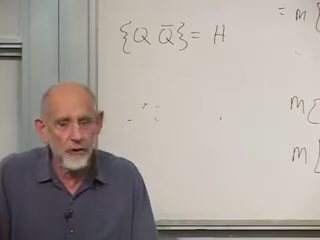
\includegraphics[width=0.62\textwidth]{lecture_05_figure_02.png}
\lectureframe{00:55:46.300}
\caption{La relación de cierre central, aislada en la pizarra. Se ven las llaves y \(Q,\bar Q,H\); la coma queda implícita en la notación habitual del anticonmutador.}
\end{figure}

Se ha elegido el cero aditivo de la energía de modo que el estado vacío tenga \(H=0\). En el oscilador supersimétrico, esta es la convención natural: las contribuciones bosónica y fermiónica de energía de punto cero se cancelan. \editorialnote{La clase trabaja directamente con la energía total en reposo y no muestra por separado los términos de punto cero; la convención indicada explicita esa elección.}

El hamiltoniano es par. También es un generador de simetría: genera traslaciones temporales. Por tanto, los generadores impares no cierran entre sí a menos que se incluya el generador par de traslaciones temporales.

\begin{classroomqa}
\audiencequestion{¿Cuál de los elementos de la relación es par? ¿Es el hamiltoniano? \lecturetimestamp{00:58:24}}
\lecturerresponse{Sí. La energía es un observable ordinario, así que \(H\) es par. La supercarga \(Q\) es impar, y el producto de dos cantidades impares es par; por consiguiente, \(\{Q,\bar Q\}\) puede ser igual a \(H\). Un generador impar y uno par se relacionan mediante un conmutador, no mediante un anticonmutador.}
\end{classroomqa}

\subsection{Completar el álgebra}

Las relaciones entre elementos de igual paridad son inmediatas:
\begin{equation}
\{Q,Q\}=2Q^2=0,
\qquad
\{\bar Q,\bar Q\}=2\bar Q^2=0,
\end{equation}
porque \(Q^2\) contiene \(c_-^2\) y \(\bar Q^2\) contiene \(c_+^2\).

Queda por establecer la relación con \(H\). Sea
\begin{equation}
H\ket{E}=E\ket{E}.
\end{equation}
Si las masas del bosón y del fermión son iguales, \(Q\) transforma uno en el otro sin cambiar la energía. Por tanto, \(Q\ket{E}\) es cero o bien otro estado propio con el mismo autovalor:
\begin{equation}
H Q\ket{E}=E Q\ket{E}.
\end{equation}
Por otro lado,
\begin{equation}
QH\ket{E}=Q(E\ket{E})=E Q\ket{E}.
\end{equation}
Al restar,
\begin{equation}
[H,Q]\ket{E}=0.
\end{equation}
Si los estados propios de la energía forman una base completa, esto vale como identidad de operadores:
\begin{equation}
[H,Q]=0,
\qquad
[H,\bar Q]=0.
\end{equation}

\begin{classroomqa}
\audiencequestion{¿Qué ocurre si el bosón y el fermión no tienen la misma masa? \lecturetimestamp{01:01:16}}
\lecturerresponse{Entonces, al sustituir uno por el otro, cambia la energía, así que la supercarga propuesta no conmuta con el hamiltoniano y se pierde la supersimetría sencilla. Para
\[
H=m_BN_B+m_FN_F,
\]
el resultado explícito es
\[
[H,Q]=(m_B-m_F)Q.
\]
Se anula precisamente cuando \(m_B=m_F\). \editorialnote{El conmutador para masas distintas expresa directamente, en forma de operador, el argumento basado en el cambio de energía y hace explícita la condición de igualdad de masas.}}
\end{classroomqa}

\begin{classroomqa}
\audiencequestion{¿Se puede repetir más despacio el argumento basado en los estados propios de la energía? \lecturetimestamp{01:01:37}}
\lecturerresponse{Partamos de \(H\ket{E}=E\ket{E}\). La igualdad de masas implica que \(Q\ket{E}\) tiene la misma energía definida \(E\), por lo que \(HQ\ket{E}=EQ\ket{E}\). En el otro orden se obtiene \(QH\ket{E}=QE\ket{E}=EQ\ket{E}\), porque \(E\) es un escalar ordinario. Su diferencia se anula en cada estado propio de la energía. La completitud permite extender la afirmación desde esos estados a la ecuación de operadores \([H,Q]=0\).}
\end{classroomqa}

Por tanto, el álgebra completa de este modelo es
\begin{align}
\{Q,\bar Q\}&=H,\\
\{Q,Q\}&=\{\bar Q,\bar Q\}=0,\\
[H,Q]&=[H,\bar Q]=0.
\end{align}
Las supercargas son cargas impares conservadas. Más sorprendentemente, su álgebra combina una operación que cambia el tipo de partícula con el generador de las traslaciones del espacio-tiempo.

\section{Por qué el hamiltoniano representa las traslaciones temporales}

En este modelo simplificado no hay coordenada espacial, pero sí hay tiempo. La ecuación de Schrödinger es
\begin{equation}
i\frac{\partial}{\partial t}\ket{\psi(t)}
=H\ket{\psi(t)}.
\end{equation}

\begin{figure}[H]
\centering
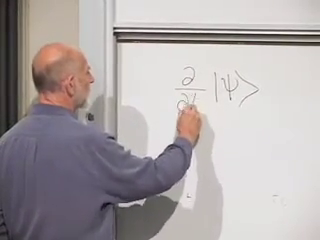
\includegraphics[width=0.56\textwidth]{lecture_05_figure_03.png}
\lectureframe{01:07:26.300}
\caption{La derivada temporal escrita junto a \(\ket{\psi}\). La mano oculta parte del denominador; la ecuación de Schrödinger completa aparece arriba.}
\end{figure}

Para un desplazamiento finito \(\delta\),
\begin{equation}
\ket{\psi(t+\delta)}
=e^{-iH\delta}\ket{\psi(t)}.
\end{equation}
Al desarrollar hasta primer orden,
\begin{equation}
\ket{\psi(t+\delta)}
=\left(\mathbf 1-i\delta H\right)\ket{\psi(t)}
+O(\delta^2).
\end{equation}
Así, \(H\) es el generador infinitesimal que actualiza el estado en el tiempo.

Las simetrías internas, como el isospín y el color, también cambian las etiquetas de las partículas. El isospín puede mezclar los estados del protón y del neutrón; las rotaciones de color mezclan los quarks rojos, verdes y azules. Sin embargo, ninguna composición de esas transformaciones internas traslada un sistema en el espacio o en el tiempo. La supersimetría es distinta:
\begin{equation}
\begin{gathered}
\text{odd particle-changing transformation}\\
\mathrel{\stackrel{\{\ ,\ \}}{\Longrightarrow}}\\
\text{time translation}
\end{gathered}
\end{equation}
Esto indica que los generadores impares podrían ser ellos mismos traslaciones, pero a lo largo de coordenadas distintas de las habituales.

\section{Superspacio}

\subsection{Una función del tiempo y de coordenadas impares}

Introduzcamos una función
\begin{equation}
\Psi=\Psi(\theta,\bar\theta,t).
\end{equation}
Puede interpretarse como una función de onda en el modelo simplificado o, en general, como un supercampo. Como el desarrollo impar se trunca,
\begin{equation}
\Psi(\theta,\bar\theta,t)
=A(t)+\bar\chi(t)\theta
+\bar\theta\chi(t)+F(t)\bar\theta\theta.
\end{equation}
Un único objeto reúne funciones componentes pares e impares. \editorialnote{Este desarrollo en componentes aplica el polinomio de Grassmann introducido antes; constituye el contenido explícito habitual de una función en el superspacio de este modelo.}

Una traslación temporal ordinaria deja fijo \(\theta,\bar\theta\) y transforma
\begin{equation}
t\longmapsto t+\delta.
\end{equation}
A primer orden,
\begin{equation}
\Psi(\theta,\bar\theta,t+\delta)
=\Psi(\theta,\bar\theta,t)
+\delta\,\partial_t\Psi(\theta,\bar\theta,t).
\end{equation}

\begin{figure}[H]
\centering
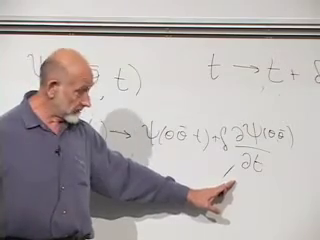
\includegraphics[width=0.72\textwidth]{lecture_05_figure_04.png}
\lectureframe{01:13:15.060}
\caption{La pizarra muestra \(t\to t+\delta\) encima del cambio de primer orden de \(\Psi\), e indica directamente el término de la derivada.}
\end{figure}

\subsection{Traslación en una dirección impar}

Inventemos ahora una transformación que desplace una coordenada impar:
\begin{equation}
\theta\longmapsto\theta+\epsilon,
\end{equation}
donde \(\epsilon\) es otro parámetro impar de Grassmann. Al mismo tiempo, hagamos que el tiempo adquiera un desplazamiento nilpotente par,
\begin{equation}
t\longmapsto t+i\bar\theta\epsilon.
\end{equation}
Tanto \(\bar\theta\) como \(\epsilon\) son impares, así que su producto es par y puede sumarse de manera coherente a la coordenada par \(t\).

Con el parámetro a la izquierda,
\begin{equation}
i\bar\theta\epsilon=-i\epsilon\bar\theta.
\end{equation}
La variación inducida es, por tanto,
\begin{align}
\delta_\epsilon\Psi
&=\epsilon\,\partial_\theta\Psi
-i\epsilon\bar\theta\,\partial_t\Psi\\
&=\epsilon q_0\Psi,
\end{align}
donde
\begin{equation}
q_0=\partial_\theta-i\bar\theta\partial_t.
\end{equation}
Este operador diferencial impar es el generador del desplazamiento combinado. Un generador conjugado compatible, con derivadas izquierdas, es
\begin{equation}
\bar q_0=-\partial_{\bar\theta}
+i\theta\partial_t.
\end{equation}

Los signos exactos dependen de si se usan derivadas izquierdas o derechas de Grassmann y de cómo la conjugación invierte los factores impares. Lo que no debe depender de la convención es el cierre sobre las traslaciones temporales. Con las definiciones anteriores,
\begin{align}
\{q_0,\bar q_0\}
&=i\{\partial_\theta,\theta\}\partial_t
+i\{\bar\theta,\partial_{\bar\theta}\}\partial_t\\
&=2i\partial_t.
\end{align}
El término con dos derivadas se anula, al igual que el término cuadrático en las coordenadas impares. Los dos términos mixtos aportan \(i\partial_t\) cada uno.

Como \(H=i\partial_t\) sobre los estados en la representación de Schrödinger,
\begin{equation}
\{q_0,\bar q_0\}=2H.
\end{equation}
Si normalizamos de modo que
\begin{equation}
q=\frac{q_0}{\sqrt2},
\qquad
\bar q=\frac{\bar q_0}{\sqrt2},
\end{equation}
entonces
\begin{equation}
\boxed{\{q,\bar q\}=H.}
\end{equation}
\editorialnote{La clase desarrolla deliberadamente los signos con cierta incertidumbre y luego observa que aparece un factor de dos. La convención mostrada para las derivadas izquierdas conserva ese cálculo en la pizarra, a la vez que fija una normalización coherente. Otras convenciones habituales trasladan los signos entre los desplazamientos de coordenadas y los generadores.}

\begin{classroomqa}
\audiencequestion{¿De dónde sale el factor final de dos en el anticonmutador del superspacio? \lecturetimestamp{01:24:21}}
\lecturerresponse{Hay dos contribuciones mixtas iguales. Una proviene de \(\{\partial_\theta,\theta\}=1\) y la otra de \(\{\partial_{\bar\theta},\bar\theta\}=1\). Cada una multiplica la derivada temporal. Por eso, para los generadores sin normalizar se obtiene \(2i\partial_t\); un factor \(1/\sqrt2\) en cada supercarga restablece la normalización anterior.}
\end{classroomqa}

\begin{classroomqa}
\audiencequestion{¿Se usó en la construcción la hipótesis de que \(\epsilon\) es pequeño? \lecturetimestamp{01:24:51}}
\lecturerresponse{Se usó la nilpotencia, no una magnitud numérica ordinaria. Como \(\epsilon^2=0\), todo desarrollo en una sola \(\epsilon\) termina tras el primer orden. Llamarla infinitesimal o pequeña es una analogía útil, pero la truncación es exacta.}
\end{classroomqa}

\editorialnote{Los parámetros de Grassmann no tienen una magnitud positiva ordinaria. Su papel como parámetros infinitesimales se debe a la nilpotencia y a la terminación exacta del desarrollo.}

\subsection{El significado geométrico}

El álgebra tiene ahora dos realizaciones equivalentes. En la descripción mediante osciladores, \(Q\) y \(\bar Q\) transforman fermiones en bosones y bosones en fermiones. En la descripción geométrica, \(q\) y \(\bar q\) trasladan una función a través de direcciones impares e inducen un desplazamiento temporal ordinario. En ambas descripciones,
\begin{equation}
\begin{gathered}
\{\text{supercharge},\text{conjugate supercharge}\}\\
=\text{time-translation generator}.
\end{gathered}
\end{equation}

El espacio de coordenadas generalizado que contiene \(t,\theta,\bar\theta\) es el superspacio. En una teoría de campos relativista también contiene las coordenadas espaciales ordinarias, y las supercargas cierran sobre el momento total del espacio-tiempo \(P_\mu\), no solo sobre \(H=P_0\). Curvar esta estructura conduce hacia la supergravedad.

En cierto sentido, las variables de Grassmann son un recurso eficiente para llevar la cuenta de bosones y fermiones. En otro, la relación de cierre expresa algo mucho más profundo: la distinción entre el tipo de partícula y la geometría del espacio-tiempo deja de ser absoluta. Desplazarse dos veces en direcciones impares produce un desplazamiento en una dirección ordinaria. Que la naturaleza realice experimentalmente esta estructura es una cuestión aparte del hecho matemático de que la estructura sea coherente, económica y extraordinariamente rígida.
